\documentclass[tikz,border=8pt]{standalone}
\usepackage{amsmath}
\usetikzlibrary{arrows.meta,positioning}

\begin{document}
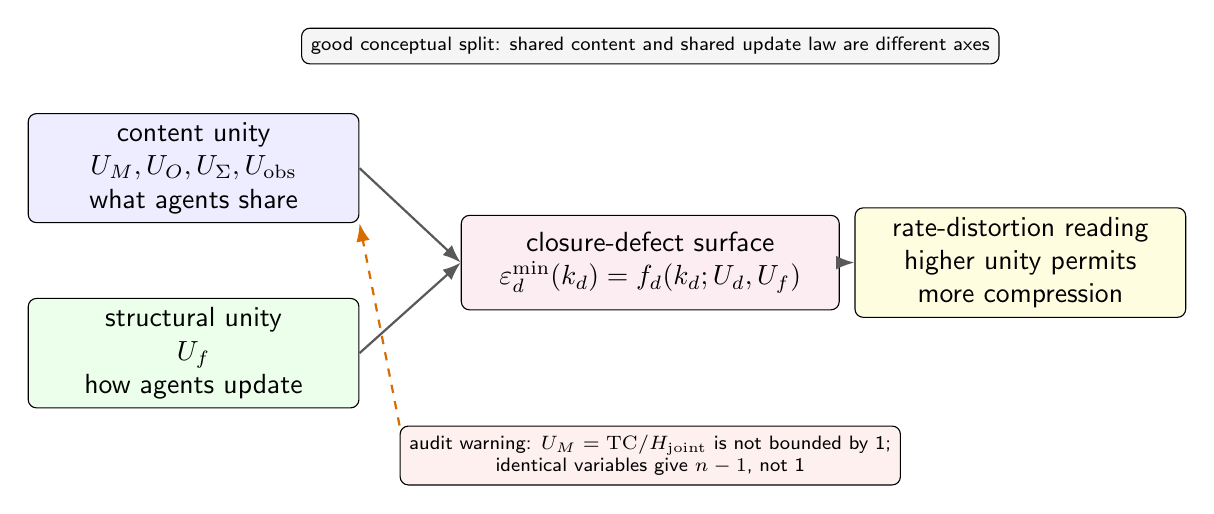
\begin{tikzpicture}[
  font=\sffamily,
  box/.style={draw, rounded corners=3pt, align=center, minimum width=42mm, minimum height=12mm, fill=white},
  note/.style={draw, rounded corners=3pt, align=center, font=\sffamily\scriptsize, fill=white},
  arrow/.style={-Latex, thick, draw=black!65},
  warn/.style={-Latex, thick, dashed, draw=orange!85!black}
]

\node[box, fill=blue!7] (content) at (-4.5,1.2)
  {content unity\\$U_M,U_O,U_\Sigma,U_{\rm obs}$\\what agents share};
\node[box, fill=green!8] (structure) at (-4.5,-1.15)
  {structural unity\\$U_f$\\how agents update};
\node[box, fill=purple!7, minimum width=48mm] (surface) at (1.3,0)
  {closure-defect surface\\$\varepsilon_d^{\min}(k_d)=f_d(k_d;U_d,U_f)$};
\node[box, fill=yellow!12] (projection) at (6.0,0)
  {rate-distortion reading\\higher unity permits\\more compression};

\draw[arrow] (content.east) -- (surface.west);
\draw[arrow] (structure.east) -- (surface.west);
\draw[arrow] (surface.east) -- (projection.west);

\node[note, fill=red!6, minimum width=63mm] (norm) at (1.3,-2.45)
  {audit warning: $U_M=\mathrm{TC}/H_{\rm joint}$ is not bounded by 1;\\identical variables give $n-1$, not 1};
\draw[warn] (norm.north west) -- (content.south east);

\node[note, fill=gray!8, minimum width=73mm] at (1.3,2.75)
  {good conceptual split: shared content and shared update law are different axes};

\end{tikzpicture}
\end{document}
